\documentclass[a4paper,12pt,twoside,final]{book}
\usepackage[utf8]{inputenc}

\usepackage[bookmarks = true, colorlinks=true, linkcolor = black, citecolor = black, menucolor = black, urlcolor = black]{hyperref}
% Nuevo
\usepackage{csquotes}

\usepackage[spanish,es-nodecimaldot]{babel} % International, rec. by RAE: http://www.tex-tipografia.com/marca_decimal.html
%\usepackage[backend=bibtex, maxbibnames=99, giveninits=true]{biblatex}
\usepackage[backend=biber, maxbibnames=99, giveninits=true]{biblatex}
\addbibresource{references.bib}
% COLOR
\usepackage[usenames,dvipsnames,svgnames,table]{xcolor}
% Colores para estilo Proyecto Docente (tonos naranjas)
\definecolor{lightback}{HTML}{F4E0BF}
     \definecolor{back}{HTML}{F3C591}
\definecolor{lightline}{HTML}{FCAF5F}
     \definecolor{line}{HTML}{ED7900}
% Colores para portada
\definecolor{epsc:oscuro}{HTML}{280091}
 \definecolor{epsc:medio}{HTML}{4C5CC5}
 \definecolor{epsc:claro}{HTML}{3FCFD5}
 \definecolor{epsc:verde}{HTML}{00B299}




\usepackage{tikz} % used in cover to place images

\usepackage{datetime} % allow formal date format
% "Month, YEAR" date format, in spanish with the month uppercased not interfering other dates
\newcommand\Monthname[1][EMPTY]{
  \ifnum1=#1Enero\else
  \ifnum2=#1Febrero\else
  \ifnum3=#1Marzo\else
  \ifnum4=#1Abril\else
  \ifnum5=#1Mayo\else
  \ifnum6=#1Junio\else
  \ifnum7=#1Julio\else
  \ifnum8=#1Agosto\else
  \ifnum9=#1Septiembre\else
  \ifnum10=#1Octubre\else
  \ifnum11=#1Noviembre\else
  \ifnum12=#1Diciembre\else
  \fi\fi\fi\fi\fi\fi\fi\fi\fi\fi\fi\fi
}
\newdateformat{monthyeardate}{%
  \Monthname[\THEMONTH], \THEYEAR}


% FONTs
\usepackage[T1]{fontenc}
\usepackage{textcomp}           % Needed for new symbols like € ?

\usepackage[scaled]{berasans} % Font for the cover similar to Vera 33
%\renewcommand*\familydefault{\sfdefault}  %% To use as the base font of the document is to be sans serif


% PAGE STYLE
\usepackage[twoside,bindingoffset=0cm,headheight=30pt,margin=25mm]{geometry} %,verbose,showframe
\usepackage{fancyhdr} % Encabezados
\pagestyle{fancy}
\fancyhf{}
\fancyhead[LE]{\leftmark}
\fancyhead[RO]{\rightmark}
\fancyfoot[RO,LE]{\thepage}
% XXX Evitar el binding en la portada pero no en el resto del documento

% Sangría para párrafo, tabulaciones de 1 cm
\parindent=1.0cm
% Espacio o separación entre párrafos
\parskip 1.5ex

% TABLES AND FIGURES
\usepackage{graphicx}
\graphicspath{ {img/} }

\usepackage{todonotes}
\usepackage{float}
\usepackage{tabularx}
\usepackage{url}
\usepackage{emptypage}
\usepackage[toc,page]{appendix}
\usepackage{hyperref}
\usepackage{array}
\usepackage{wrapfig}
\usepackage{multirow}
\usepackage{multicol} %Para poner columnas de un solo elemento
\usepackage{tabu}
\usepackage{tikz}

\usepackage{pifont} %Para usar el vmark (tick) y xmark (cross)
\newcommand{\vmark}{\textcolor{green}{\ding{51}}} %Definición del vmark en verde
\newcommand{\xmark}{\textcolor{red}{\ding{55}}} %Definición del xmark en rojo

\usepackage{chngcntr}
\usepackage{verbatim}
\usepackage{graphicx}
\usepackage[export]{adjustbox}
\usepackage{listings}


\usepackage{booktabs,caption}
\usepackage[flushleft]{threeparttable}
\usepackage{fancyvrb}
\usepackage{verbatimbox}
\usepackage{afterpage}


\newsavebox{\FVerbBox}
\newenvironment{FVerbatim}
 {\VerbatimEnvironment
  \begin{center}
  \begin{lrbox}{\FVerbBox}
  \begin{BVerbatim}}
 {\end{BVerbatim}
  \end{lrbox}
  \fbox{\usebox{\FVerbBox}}
  \end{center}}
  
  
  \newcommand\blankpage{%
    \null
    \thispagestyle{empty}%
    \addtocounter{page}{-1}%
    \newpage}
    
\counterwithout{footnote}{chapter}
  
\begin{document}
\frontmatter

%------------- Cover --------------
\thispagestyle{empty}

% Backgroud images
\begin{tikzpicture}[remember picture, overlay]
  % Top
  \node [anchor=north east, inner sep=0pt]  at (current page.north east)
     {
\includegraphics[height=6cm]{topRightCorner.pdf}};
  % Bottom
  \node [anchor=south west, inner sep=0pt]  at (current page.south west)
     {
\includegraphics[height=6cm]{bottomLeftCorner.pdf}};
  \node (uco) [anchor=south east, inner sep=0pt, xshift=-10mm, yshift=10mm]  at (current page.south east)
        {
\includegraphics[height=2cm]{uco_debajo.pdf}};
  \node [anchor=south east, inner sep=0pt, xshift=-10mm]  at (uco.south west)
% Uncomment the chosen logo and comment the others:
        {
\includegraphics[height=2cm]{emblema-ing-informatica.pdf}};
%        {
\includegraphics[height=2cm]{emblema-ing-industrial.pdf}};
%        {
\includegraphics[height=2cm]{emblema-ing-tec-industrial.pdf}};
\end{tikzpicture}

\renewcommand*\listtablename{Índice de tablas}
\renewcommand{\tablename}{Tabla}
\begin{center}
\fontfamily{\sfdefault}\selectfont
\vspace*{2cm}

\vfill
\vfill

\includegraphics[width=12.5cm]{LogotipoEPSC.pdf}
\vfill
\vfill

\large\textbf{\color{epsc:medio}
  TRABAJO FIN DE GRADO
}
\vfill

\Large\textbf{\color{epsc:verde}
  Grado en Ingeniería Informática
}
\vfill
\large\textbf{\color{epsc:verde}
 Especialidad de Ingeniería del Software
}
\vfill

\Huge\textbf{\color{epsc:oscuro}
  Aplicación web para la gestión de comisiones de los centros pertenecientes a la Universidad de Córdoba
  }
\vfill
\vfill
\Large\textbf{\color{epsc:verde}
  Petición de tema
}
\vfill
\vfill


\large{\color{epsc:oscuro}Autor}\\
\textbf{\color{epsc:medio}{ Javier Ruiz Jurado }}
\vfill

\large{\color{epsc:oscuro} Director }\\
\textbf{\color{epsc:medio} Prof. Dr. José Luis Ávila Jiménez }
\vfill



\textbf{\color{epsc:verde} \monthyeardate\today}
\vfill
\vfill
\vspace{2.7cm}
\end{center}


%-------------------------------------------------------------------------------------------------------
\cleardoublepage
\setcounter{page}{1}
\tableofcontents
\listoffigures
\listoftables
%\cleardoublepage

\afterpage{\null\newpage}
\thispagestyle{empty}
\newpage
\mainmatter
%Insertar capitulos
\chapter{Introducción}

\section{Comisiones de centros de la Universidad de Córdoba}

La Universidad de Córdoba (UCO)\cite{uco} es una institución universitaria localizada en la ciudad de Córdoba y fundada en el año 1972. La UCO cuenta actualmente con un total de diez centros propios, dos centros adscritos, el Instituto de Estudios de Posgrado (IDEP) y el Centro Intergeneracional ``Francisco Santisteban''. Los centros propios están organizados en cuatro Campus universitarios: tres en la ciudad y uno en Belmez.
   \begin{itemize}
    \item \textbf{Centros propios}
        \begin{itemize}
        \item Facultades:
            \begin{itemize}
                \item Facultad de Ciencias (Campus de Rabanales).
                \item Facultad de Ciencias de la Educación y Psicología (Campus de Menéndez Pidal).
                \item Facultad de Ciencias del Trabajo  (Campus del Centro Histórico).
                \item Facultad de Derecho y Ciencias Económicas y Empresariales (Campus del Centro Histórico).
                \item Facultad de Filosofía y Letras (Campus del Centro Histórico).
                \item Facultad de Medicina y Enfermería  (Campus de Menéndez Pidal).
                \item Facultad de Veterinaria (Campus de Rabanales).
            \end{itemize}
        \item Escuelas:
        \begin{itemize}
            \item Escuela Politécnica Superior de Belmez (Campus de Belmez).
            \item Escuela Politécnica Superior de Córdoba (Campus de Rabanales).
            \item Escuela Técnica Superior de Ingeniería Agronómica y de Montes (Campus de Rabanales).
        \end{itemize}
    \end{itemize}
    \item \textbf{Centros adscritos}
    \begin{itemize}
        \item Centro de Magisterio ``Sagrado Corazón'', con sede en Córdoba.
        \item Centro Universitario FIDISEC, con sede en Cabra.
    \end{itemize}
\end{itemize}    

Cada uno de estos centros, ya sea facultad o escuela, actúan para el cumplimiento de sus fines a través de los siguientes órganos de gobierno y representación, formando el \textbf{Equipo de Gobierno} del centro \cite{reglamento}: 
\begin{itemize}
    \item \textbf{Junta de Centro o Escuela}: es el órgano colegiado de gobierno, que ejerce sus funciones con sujeción a los acuerdos del Equipo de Gobierno y a las resoluciones del Rector, de acuerdo con lo establecido en los Estatutos de la Universidad de Córdoba y en el actual Reglamento. Entre sus funciones principales, se encarga de tomar las decisiones y establecer las políticas académicas y administrativas del centro.
    \item \textbf{Decano o Director}: ostenta la representación de la Facultad o Escuela, respectivamente, y ejerce las funciones de dirección y gestión ordinaria de la misma. 
    \item \textbf{Vicedecanos o Subdirectores}: el Decano o Director podrá proponer, para su nombramiento por el Rector, a Vicedecanos o Subdirectores, respectivamente, entre los profesores con vinculación permanente a la universidad adscritos al Centro, en los que podrá delegar funciones que le son propias

    \item \textbf{Secretario}: será nombrado por el Rector, a propuesta del Decano o Director, entre los profesores con vinculación permanente a la Universidad de Córdoba adscritos al Centro, en los que podrá delegar funciones que le son propias.

\end{itemize}

La Junta de Centro o Escuela podrá crear cuantas Comisiones considere necesarias para el buen desarrollo de sus funciones. Las \textbf{Comisiones} son grupos de trabajo especializados que se crean dentro del centro para abordar temas específicos, como la planificación curricular, la investigación o la gestión de recursos. Los miembros de estas Comisiones serán elegidos o designados por la Junta de Centro o Escuela entre personal docente e investigador, personal de administración y servicios y estudiantes, atendiendo a la naturaleza de la Comisión.

Existirán al menos las siguientes Comisiones en cada centro:
\begin{itemize}
    \item Comisión de Asuntos Económicos.
    \item Comisión de Docencia.
    \item Comisión de Ordenación Académica.
    \item Comisión de Relaciones Exteriores.
    \item Comisión de Reconocimientos y Convalidaciones.
    \item Comisión Académica de los Másteres.
    \item Unidades de Garantía de Calidad.
\end{itemize}
    
\section{Definición del problema real}
    
    Existe un problema generalizado con respecto a la gestión de las comisiones de los distintos centros pertenecientes a la Universidad de Córdoba, el cual viene dado principalmente por la ausencia de un sistema informático de gestión.
    
    Actualmente, se realizan tareas manuales y estáticas sobre estas comisiones que provocan que la gestión administrativa sobre ellas sea una tarea lenta de realizar, sin conseguir una trazabilidad de los movimientos de altas/bajas de sus miembros, pérdida de tiempo con respecto a utilizar un sistema que automatice lo máximo posible alguna de sus gestiones...

    En resumen, el problema real que se desea resolver con el desarrollo de este Trabajo de Fin de Grado es el siguiente: los centros (facultades y escuelas) de la Universidad de Córdoba no poseen una aplicación informática que permita la gestión de sus comisiones universitarias.
    
 
\section{Definición del problema técnico}

    Se va a utilizar la metodología denominada \textit{Product Design Specification} (PDS) para describir el problema técnico que se desea resolver. Esta metodología permite dar respuesta a una serie de apartados que se enumeran a continuación.
    
\subsection{Funcionamiento}
    Se desea implementar una aplicación web que permita realizar una gestión de las comisiones pertenecientes a los centros de la Universidad de Córdoba. 
    
    Los usuarios que interactuarán con la aplicación son los siguientes:
    \begin{itemize}
        \item Administrador
          \begin{itemize}
              \item Este tipo de usuario estará registrado en el sistema y tendrá un control completo de la aplicación. 
              \item En particular, tendrá las competencias exclusivas de la gestión de todos los tipos de usuarios, centros, juntas, miembros y comisiones. Además, se encargará de la gestión de las copias de seguridad.
          \end{itemize}
          \item Responsable del centro
           \begin{itemize}
               \item Este tipo de usuario estará registrado en el sistema y representará a una persona que podrá gestionar la información de un centro.
               \item En particular, tendrá las competencias exclusivas de la asignación/exclusión a los miembros de gobierno pertenecientes a dicho centro, de creación de las juntas que pertenezcan al centro, así como asignación/exclusión del responsable de cada junta.
            \end{itemize}
            \item Responsable de la junta
           \begin{itemize}
               \item Este tipo de usuario estará registrado en el sistema y representará a una persona que podrá gestionar la información de una junta de centro.
               \item En particular, tendrá las competencias exclusivas de la asignación/exclusión a los miembros de junta pertenecientes a dicha junta, de la gestión de las convocatorias realizadas por la junta, de los miembros que participarán en cada una de las convocatorias de la junta, de creación de las comisiones que pertenezcan a la junta, así como asignación/exclusión del responsable de cada comisión.
            \end{itemize}
          \item Responsable de la comisión 
           \begin{itemize}
               \item Este tipo de usuario estará registrado en el sistema y representará a una persona que podrá gestionar la información de una comisión.
               \item En particular, tendrá las competencias exclusivas de la asignación/exclusión a los miembros pertenecientes a dicha comisión, gestión de las convocatorias realizadas por la comisión, y de los miembros que participarán en cada una de las convocatorias de dicha comisión.
            \end{itemize}
        \item Usuario universitario
            \begin{itemize}
                \item Este tipo de usuario estará registrado en el sistema.
                \item Podrá obtener distintos certificados como pueden ser de situación actual, de centros en los que ha participado como miembro de equipo de gobierno, de juntas a las que ha representado, de comisiones a las que ha pertenecido, de convocatorias en las que ha participado...
              \end{itemize}
        \item Público
        \begin{itemize}
              \item Este tipo de usuario no necesitará estar registrado en el sistema.
              \item Podrá consultar la información pública disponible: comisiones de un centro, miembros actuales de una comisión, consulta de actas aprobadas y pendientes de aprobación,...
          \end{itemize}
     \end{itemize}
     
\subsection{Entorno}
 Existirán dos entornos de trabajo para esta aplicación. 

  \begin{itemize}
     \item Entorno de desarrollo y testeo: entorno que se utilizará para desarrollar, probar y depurar la aplicación web antes de su lanzamiento al entorno de producción.
     \item Entorno de producción:
         entorno en el que se encontrará la versión final de la aplicación web, una vez de pasadas todas las pruebas y correcciones necesarias en el entorno de desarrollo y pruebas. Estará configurado y optimizado para garantizar un rendimiento y disponibilidad óptimos, así como protegido por diferentes medidas de seguridad.
 \end{itemize}

Existirán dos entornos de ejecución para esta aplicación. 

 \begin{itemize}
     \item Entorno de ejecución del administrador:
         el administrador ejecutará la aplicación desde un servidor que le permitirá acceder a todos los recursos de software y así poder modificar cualquier aspecto del sistema.
     \item Entorno de ejecución de los demás usuarios:
         el resto de usuarios (público, registrado, responsable del centro,junta y comisión y miembro de gobierno, junta y comisión) ejecutarán la aplicación desde su propios equipos, siempre que estos tengan conexión a internet al tratarse de una aplicación web.
 \end{itemize}

 La interfaz es el medio de comunicación entre los usuarios y la aplicación web. Es importante que la interfaz sea lo más intuitiva y amigable posible para poder generar una mejor experiencia en el usuario. Los requisitos de la interfaz se describirán en la Sección Requisitos de la interfaz.

 La aplicación web será completamente responsiva, adaptándose a a diferentes tamaños y resoluciones de pantalla de diferentes dispositivos, como móviles, tabletas, ordenadores de escritorio,...

En resumen, una aplicación web responsiva nos brindará una experiencia de usuario cómoda y consistente en todos los dispositivos, mejorando la accesibilidad de la aplicación así como su visibilidad en línea.

        
\subsection{Vida esperada}
    
    El ciclo de vida esperado para dicha aplicación web será alto ya que se considera que prácticamente no van a cambiar las tareas comunes de la gestión de comisiones.
    
    Sin embargo, sí es posible que haya que actualizar la aplicación web debido a la aparición de nuevos recursos de software o hardware, o versiones mejoradas de los mismos, que puedan mejorar la aplicación web que se desea desarrollar: rendimiento, seguridad, etc.
    
\subsection{Ciclo de mantenimiento} \label{subsec:ciclo_mantenimiento}

 Teniendo en cuenta que el propósito de la creación de esta aplicación web es la realización de un Trabajo de Fin de Grado, el mantenimiento de dicha aplicación no correrá a cargo de su autor.

 No obstante, se realizará un diseño modular de cada una de las partes de la aplicación web para facilitar, en el futuro, posibles tareas de mantenimiento y mejoras.


\subsection{Competencia}

 No procede realizar un posible análisis de competencia comercial puesto que se trata del desarrollo de una aplicación web con fines educativos, teniendo como objetivo final el desarrollo de un Trabajo de Fin de Grado.

 Además, no se tiene conocimiento de que la Universidad de Córdoba disponga de una aplicación web para la gestión de las comisiones de sus centros universitarios. Tampoco se conoce la existencia de aplicaciones similares en otras universidades.


\subsection{Aspecto externo}

En relación con el aspecto externo, se tendrán en cuenta los siguientes aspectos:

\begin{itemize}
    \item \textbf{Interfaz de usuario}
    \begin{itemize}
        \item Se realizará una interfaz totalmente responsiva, intuitiva y amigable para que el usuario pueda navegar de la manera más cómoda posible. El Capítulo Diseño de la interfaz describirá el Diseño de la Interfaz de la aplicación web que se va  a desarrollar.
    \end{itemize}
    \item \textbf{Distribución de la aplicación: formato de almacenamiento}
     \begin{itemize}
         \item La aplicación se podrá distribuir a través de un repositorio en la nube.
     \end{itemize}
     
    \item \textbf{Documentación}
     \begin{itemize}
         \item Se elaborarán los siguientes manuales:
        \begin{itemize}
        \item Manual técnico: este documento en el que describirán todas las fases de desarrollo de la aplicación web.
        \item Manual del usuario: describirá la instalación y desinstalación de la aplicación web y las indicaciones para su utilización por los diferentes tipos de usuarios
        \item Manual de código: constará de dos partes. La documentación externa describirá los recursos de hardware y software utilizados, y agrupará el código en bloques funcionales (interfaz, base de datos, etc.). La documentación interna comentará los ficheros de código.
    \end{itemize}
     \end{itemize}
\end{itemize}


\subsection{Estandarización}

 Para el desarrollo de la aplicación web, se revisarán las 
 las recomendaciones propuestas por \textit{World Wide Web Consortium} (W3C) \cite{w3c}, que ``promueve el uso de estándares para reducir el coste y la complejidad del desarrollo, así como para incrementar la accesibilidad y usabilidad de cualquier documento publicado en la web'' \cite{revistadigital}.

 También se debe tener en cuenta que los recursos  que se van a utilizar son herramientas informáticas que están validadas por prestigiosas organizaciones que indican que cumplen con los estándares. Véase el capítulo \ref{cap:recursos} de Recursos. 

\subsection{Calidad y fiabilidad}

 La calidad y la fiabilidad de la aplicación web estará garantizadas por las siguientes razones.
 \begin{itemize}
     \item Se va a utilizar una metodología de Ingeniería del Software para especificar los requisitos (funcionales, no funcionales, de información y de la interfaz), modelar la información que se va a utilizar, analizar las funciones que se van a desarrollar, diseñar el modelo de datos, clases y paquetes, diseñar la interfaz, etc. 
     \item Se van a utilizar recursos de software ampliamente usados y contrastados en el desarrollo de aplicaciones web.
     \item La aplicación web será sometida a un completo proceso de pruebas para comprobar que es correcta, robusta y amigable.
 \end{itemize}

\subsection{Programa de tareas}

 El desarrollo del presente Trabajo de Fin de Grado va estar compuesto por la siguientes fases:
 \begin{itemize}
     \item Introducción: descripción del problema, establecimiento de los objetivos, revisión de antecedentes, identificación de restricciones iniciales y estratégicas y selección de recursos.
     \item Análisis: especificación de requisitos (funcionales, no funcionales, de información y de la interfaz), descripción del modelo de datos y análisis funcional (casos de uso y diagramas de secuencia).
    
     \item Diseño: descripción del diseño de datos, clases, paquetes y de la interfaz.
    
     \item Implementación: codificación de la aplicación web teniendo en cuenta el diseño desarrollado.
    
     \item Pruebas: comprobación de que la aplicación web funciona correctamente, es robusta y amigable.
    
     \item Documentación: redacción del manual técnico (este documento), el manual de usuario y el manual de código.
 \end{itemize}


\subsection{Pruebas}

La fase de pruebas es esencial para garantizar que la aplicación web funciona correctamente. En particular, se pretende comprobar que la aplicación web:
\begin{itemize}
    \item Hace lo que debe hacer.
    \item No provoca efectos secundarios que pueden desencadenar situaciones catastróficas.
    \item Contiene módulos que se ejecutan correctamente.
    \item Garantiza los privilegios de cada tipo de usuario.
\end{itemize}

Cada prueba tendrá la siguiente estructura para detectar los errores y corregirlos:
\begin{itemize}
    \item Objetivo de la prueba. Se debe indicar en qué consiste la prueba y el resultado esperado.
    \item Problema detectado, en su caso. Si ocurre un error entonces se debe describir la causa que lo ha provocado.
    \item Solución adoptada, en su caso. Si se ha producido un error, se deben indicar las medidas tomadas para solucionarlo.
\end{itemize}

El Capítulo de Pruebas describirá las pruebas realizadas.

\subsection{Seguridad}

Hay varias consideraciones de seguridad que se deben tener en cuenta al desarrollar una aplicación web moderna. Algunas de las más importantes son:

\begin{itemize}
    \item Autenticación y autorización: es importante garantizar que los usuarios sean autenticados correctamente antes de permitirles el acceso a diferentes vistas de la aplicación. Además, es necesario asegurarse de que los usuarios solamente tengan los permisos necesarios para realizar acciones específicas dependiendo del tipo de usuario autenticado. Además, se utilizará el control de sesiones para garantizar que un usuario no puede acceder directamente a una página web de la aplicación tecleando su dirección url si antes no se ha identificado con su clave y contraseña.

    \item Protección contra ataques de inyección: Las aplicaciones web modernas pueden ser vulnerables a ataques de inyección, como inyección de SQL o inyección de código. Es importante utilizar técnicas de validación y filtrado de datos para proteger la aplicación de estos ataques.

    \item Protección de datos: para garantizar la confidencialidad de información que establece la Ley Orgánica de Protección de Datos (LOPD) \cite{lopd}, es importante asegurarse de que los datos sensibles estén cifrados y de que la aplicación esté protegida contra la exposición de datos confidenciales.
\end{itemize}



\chapter{Objetivos}
\section{Objetivo principal}
 El objetivo de este Trabajo de Fin de Grado es el desarrollo de una aplicación web para la gestión de las comisiones de los centros de la Universidad de Córdoba: facultades y escuelas superiores. En particular, se desea gestionar la información de sus juntas de centro o juntas de escuela y de las comisiones delegadas de las mismas, como las comisiones de docencia, planes de estudios, asuntos económicos, etc.

\section{Objetivos específicos}

Los objetivos específicos de este Trabajo de Fin de Grado son los siguientes:

\begin{itemize}
    \item \textbf{Tipos de usuarios}
    \item[] Se deberán permitir los siguientes tipos de usuarios: 
     \begin{itemize}
        \item Administrador
          \begin{itemize}
              \item Este tipo de usuario estará registrado en el sistema y tendrá un control completo de la aplicación. 
              \item En particular, tendrá las competencias exclusivas de la gestión de todos los tipos de usuarios, centros, juntas, miembros y comisiones. Además, se encargará de la gestión de las copias de seguridad.
          \end{itemize}
          \item Responsable del centro
           \begin{itemize}
               \item Este tipo de usuario estará registrado en el sistema y representará a una persona que podrá gestionar la información de un centro.
               \item En particular, tendrá las competencias exclusivas de la asignación/exclusión a los miembros de gobierno pertenecientes a dicho centro, de creación de las juntas que pertenezcan al centro, así como asignación/exclusión del responsable de cada junta.
            \end{itemize}
            \item Responsable de la junta
           \begin{itemize}
               \item Este tipo de usuario estará registrado en el sistema y representará a una persona que podrá gestionar la información de una junta de centro.
               \item En particular, tendrá las competencias exclusivas de la asignación/exclusión a los miembros de junta pertenecientes a dicha junta, de la gestión de las convocatorias realizadas por la junta, de los miembros que participarán en cada una de las convocatorias de la junta, de creación de las comisiones que pertenezcan a la junta, así como asignación/exclusión del responsable de cada comisión.
            \end{itemize}
          \item Responsable de la comisión 
           \begin{itemize}
               \item Este tipo de usuario estará registrado en el sistema y representará a una persona que podrá gestionar la información de una comisión.
               \item En particular, tendrá las competencias exclusivas de la asignación/exclusión a los miembros pertenecientes a dicha comisión, gestión de las convocatorias realizadas por la comisión, y de los miembros que participarán en cada una de las convocatorias de dicha comisión.
            \end{itemize}
        \item Usuario universitario
            \begin{itemize}
                \item Este tipo de usuario estará registrado en el sistema.
                \item Podrá obtener distintos certificados como pueden ser de situación actual, de centros en los que ha participado como miembro de equipo de gobierno, de juntas a las que ha representado, de comisiones a las que ha pertenecido, de convocatorias en las que ha participado...
              \end{itemize}
        \item Público
        \begin{itemize}
              \item Este tipo de usuario no necesitará estar registrado en el sistema.
              \item Podrá consultar la información pública disponible: comisiones de un centro, miembros actuales de una comisión, consulta de actas aprobadas y pendientes de aprobación,...
          \end{itemize}
     \end{itemize}
    \item \textbf{Bases de datos relacional}
     \item[] Se deberá diseñar una base de datos relacional que permita gestionar toda la información relacionada con los centros, juntas, comisiones, convocatorias y miembros de gobierno, junta y comisión:
      \begin{itemize}
            \item Usuarios registrados: administrador, responsable centro, responsable junta comisión y usuario registrado.
            \item Centros docentes de la Universidad de Córdoba: Facultades y Escuelas.
            \item Juntas de centro o facultad: fecha constitución, fecha disolución.
            \item Comisiones: 
                \begin{itemize}
                    \item Comisión de Asuntos Económicos.
                    \item Comisión de Docencia.
                    \item Comisión de Ordenación Académica.
                    \item Comisión de Relaciones Exteriores.
                    \item Comisión de Reconocimientos y Convalidaciones.
                    \item Comisión Académica de los Másteres.
                    \item Unidades de Garantía de Calidad.
                    \item Etc.
                \end{itemize}
          \item Convocatorias de juntas y comisiones: sesión ordinaria, sesión extraordinaria.
          \item Miembro de gobierno, junta y comisión: Director, Vicedirector, profesorado permanente, PAS, alumnado...
      \end{itemize}
    \item \textbf{Módulos}
     \item[] Se deberán diseñar los siguiente módulos principales: 
        \begin{itemize}
            \item Módulo del administrador
                \begin{itemize}
                    \item Gestión de usuarios registrados: responsables y miembros de la comisión
                    \item Gestión de los centros universitarios.
                    \item Gestión de copias de seguridad
                    \item Consultar la ayuda del administrador.
                \end{itemize}

            \item Módulo del responsable de centro
                \begin{itemize}
                    \item Consultar, insertar, actualizar y eliminar la información del centro responsable.
                    \item Consultar, insertar, actualizar y eliminar la información de las juntas del centro.
                    \item Asignar/excluir miembros de gobierno del centro responsable.
                    \item Asignar/excluir responsable de las juntas del centro responsable.
                \item Consultar la ayuda del responsable de centro.
                \end{itemize}

             \item Módulo del responsable de junta
                \begin{itemize}
                    \item Consultar, insertar, actualizar y eliminar la información de la junta responsable.
                    \item Consultar, insertar, actualizar y eliminar la información de las comisiones de la junta.
                    \item Asignar/excluir miembros de las juntas del centro responsable.
                    \item Asignar/excluir responsable de las comisiones de la junta responsable.
                    \item Consultar, insertar, actualizar y eliminar la información de las convocatorias de la junta responsable.
                \item Consultar la ayuda del responsable de junta.
                \end{itemize}

             \item Módulo del responsable de comisión
                \begin{itemize}
                    \item Consultar, insertar, actualizar y eliminar la información de la comisión responsable.
                    \item Asignar/excluir miembros de las comisiones responsables.
                    \item Consultar, insertar, actualizar y eliminar la información de las convocatorias de la comisión responsable.
                \item Consultar la ayuda del responsable de comisión.
                \end{itemize}

            \item Módulo del usuario universitario.
                \begin{itemize}
                    \item Obtención de diferentes tipos certificados (pertenencia a una comisión, comisiones en las cuales ha pertenecido en un rango de fechas...).
                \item Consultar la ayuda del usuario universitario.
                \end{itemize}
         
         \item Módulo público
            \begin{itemize}
                \item Consultar la información pública: equipo de gobierno de un centro, juntas de un centro, comisiones de una junta, miembros actuales de gobierno, junta, de una comisión,...
                \item Consultar la ayuda del usuario público.
            \end{itemize}
        
        \end{itemize}
     
    \item \textbf{Diseño de la interfaz}
    \item[] Se deberá diseñar una interfaz intuitiva, robusta, amigable y adaptable a los distintos navegadores web.

    \item \textbf{Documentación}
    \item[] Se deberá redactar la siguiente documentación: manual técnico, manual de usuario y manual de código.
\end{itemize}

    
\section{Objetivos personales}

Se proponen los siguientes objetivos personales:
 \begin{itemize}
    \item Aprender y afianzar conocimientos sobre el entorno de desarrollo web Wamp \cite{wamp}, que permite instalar y configurar un servidor web en un entorno local que será utilizado como entorno de desarrollo y testeo de nuestra aplicación web.
    \item Aprender y afianzar conocimientos sobre la contratación y configuración de del \textit{hosting} VPS \cite{vps}, que será utilizado como entorno de producción, así como la utilización y configuración de dicho \textit{hosting} haciendo uso del panel de control Plesk \cite{plesk}.
    \item Aprender y afianzar conocimientos sobre el sistema de gestión de versiones Git \cite{git} para controlar todos nuestros cambios de la aplicación web en un repositorio local y remoto.
    \item Aprender y afianzar conocimientos sobre las herramientas y recursos que nos brinda el \textit{framework} denominado ``Laravel'' \cite{laravel} para el desarrollo de aplicaciones web modernas.
    \item  Aprender y afianzar conocimientos sobre el funcionamiento del gestor de bases de datos MySql \cite{mysql}.
    \item Familiarizarse con la herramienta Overleaf \cite{overleaf} para la edición de documentos en \LaTeX.   
     \item  Aprender y afianzar conocimientos sobre el \textit{framework} ''Tailwind CSS'' \cite{tailwind} para el diseño de la aplicación web.
     \item  Aprender y afianzar conocimientos sobre diferentes librerías como ''Orgchart JS'' \cite{orgchart} para la creación de organigramas interactivos.
 \end{itemize}
    
    
    
\chapter{Antecedentes}\label{cap:antecedentes}

\section{Comisiones de centros en la Universidad de Córdoba}

\section{Gestión actual de las comisiones en la Universidad de Córdoba}

La Universidad de Córdoba posee actualmente diferentes páginas web estáticas que muestran las distintas comisiones de cada uno de los centros:
    
   \begin{itemize}
    \item \textbf{Centros propios}
        \begin{itemize}
        \item Facultades:
            \begin{itemize}
                \item Facultad de Ciencias (Campus de Rabanales) \cite{WebComisionesFacultadCiencias}.
                \item Facultad de Ciencias de la Educación y Psicología (Campus de Menéndez Pidal) \cite{WebComisionesFacultadEducación}.
                \item Facultad de Ciencias del Trabajo (Campus del Centro Histórico) \cite{WebComisionesFacultadTrabajo}.
                \item Facultad de Derecho y Ciencias Económicas y Empresariales (Campus del Centro Histórico) \cite{WebComisionesFacultadEconómicas}.
                \item Facultad de Filosofía y Letras (Campus del Centro Histórico) \cite{WebComisionesFacultadFilosofía}.
                \item Facultad de Medicina y Enfermería  (Campus de Menéndez Pidal) \cite{WebComisionesFacultadMedicina}.
                \item Facultad de Veterinaria (Campus de Rabanales) \cite{WebComisionesFacultadVeterinaria}.
            \end{itemize}
        \item Escuelas:
        \begin{itemize}
            \item Escuela Politécnica Superior de Belmez (Campus de Belmez) \cite{WebComisionesEPSBelmez}.
            \item Escuela Politécnica Superior de Córdoba (Campus de Rabanales) \cite{WebComisionesEPSUco}.
            \item Escuela Técnica Superior de Ingeniería Agronómica y de Montes (Campus de Rabanales) \cite{WebComisionesEPSAgronómica}.
        \end{itemize}
    \end{itemize}
    \item \textbf{Centros adscritos}
    \begin{itemize}
        \item Centro de Magisterio ``Sagrado Corazón'', con sede en Córdoba. \cite{WebComisionesAdscritoMagisterio}
        \item Centro Universitario FIDISEC, con sede en Cabra. \cite{WebComisionesAdscritoFidisecUCO}
    \end{itemize}
\end{itemize}    

En general, estas páginas web muestran información estática de las comisiones de cada uno de los centros de la Universidad de Córdoba, siendo actualizada manualmente por parte del personal administrativo, indicando en algunos casos la fecha de la última actualización que se ha realizado. Esto implica que no es posible guardar ningún tipo de información histórica de la comisión, como por ejemplo, un cambio de miembros de la comisión, no siendo posible conocer la información de los miembros de una comisión entre unas fechas determinadas. 

Además, cualquier cambio que se realice manualmente en una página web estática puede afectar a otras  páginas relacionadas, lo que puede provocar que la  información esté duplicada, no sea consistente o no sea precisa y, por tanto, no confiable, dando a lugar a un sistema desastroso con información incorrecta.


Las Figuras  \ref{fig:WebComisionesEPSUCO} y \ref{fig:PACE-WebEquipoGobiernoEPSUCO} muestran,  a modo de ejemplo, dos páginas web en las que se repite información de datos de los nombres de los miembros que pertenecen a una comisión. Esta información ha sido introducida de manera manual e individual en cada una de las páginas. Por tanto, si se debe introducir la misma información en diferentes páginas web entonces se pueden producir errores de integridad de información.

\begin{figure}[H]
    \centering
    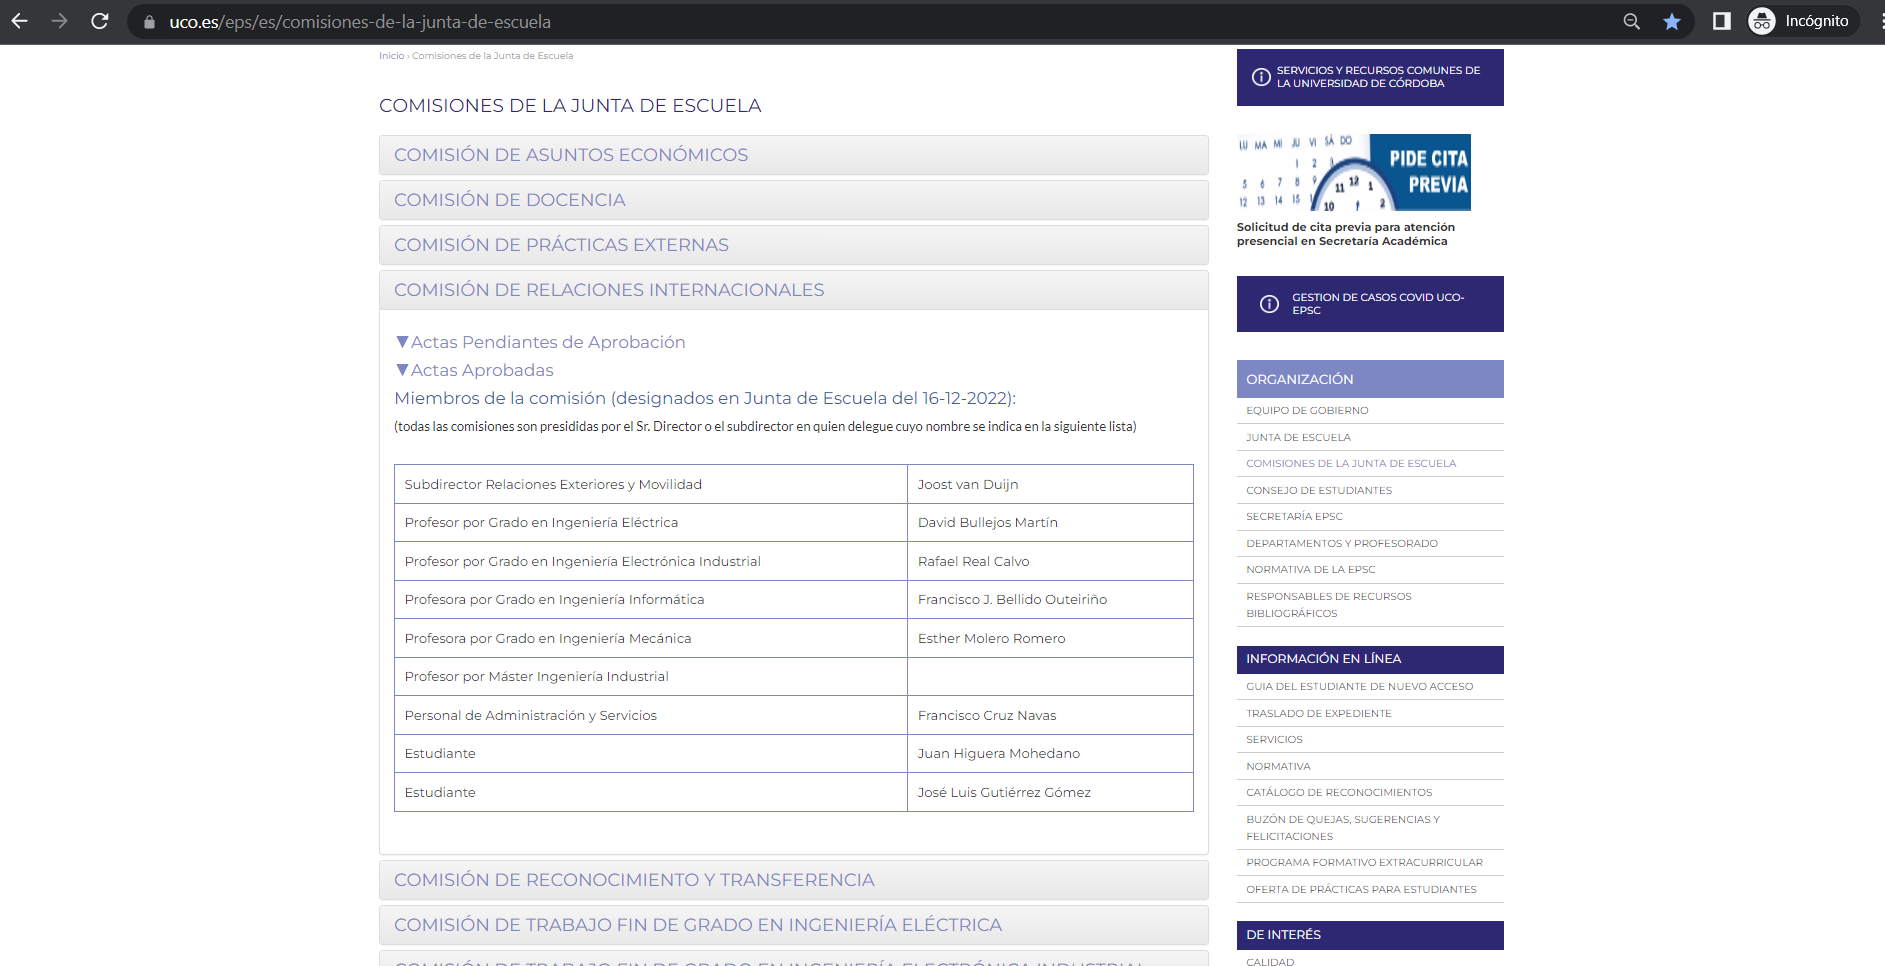
\includegraphics[scale=0.4]{img/capturas/WebComisionesEPSUCO.png}
    \caption{WEB: Información sobre los miembros de las comisiones de la EPS de la UCO}
    \label{fig:WebComisionesEPSUCO}
\end{figure}

\begin{figure}[H]
    \centering
    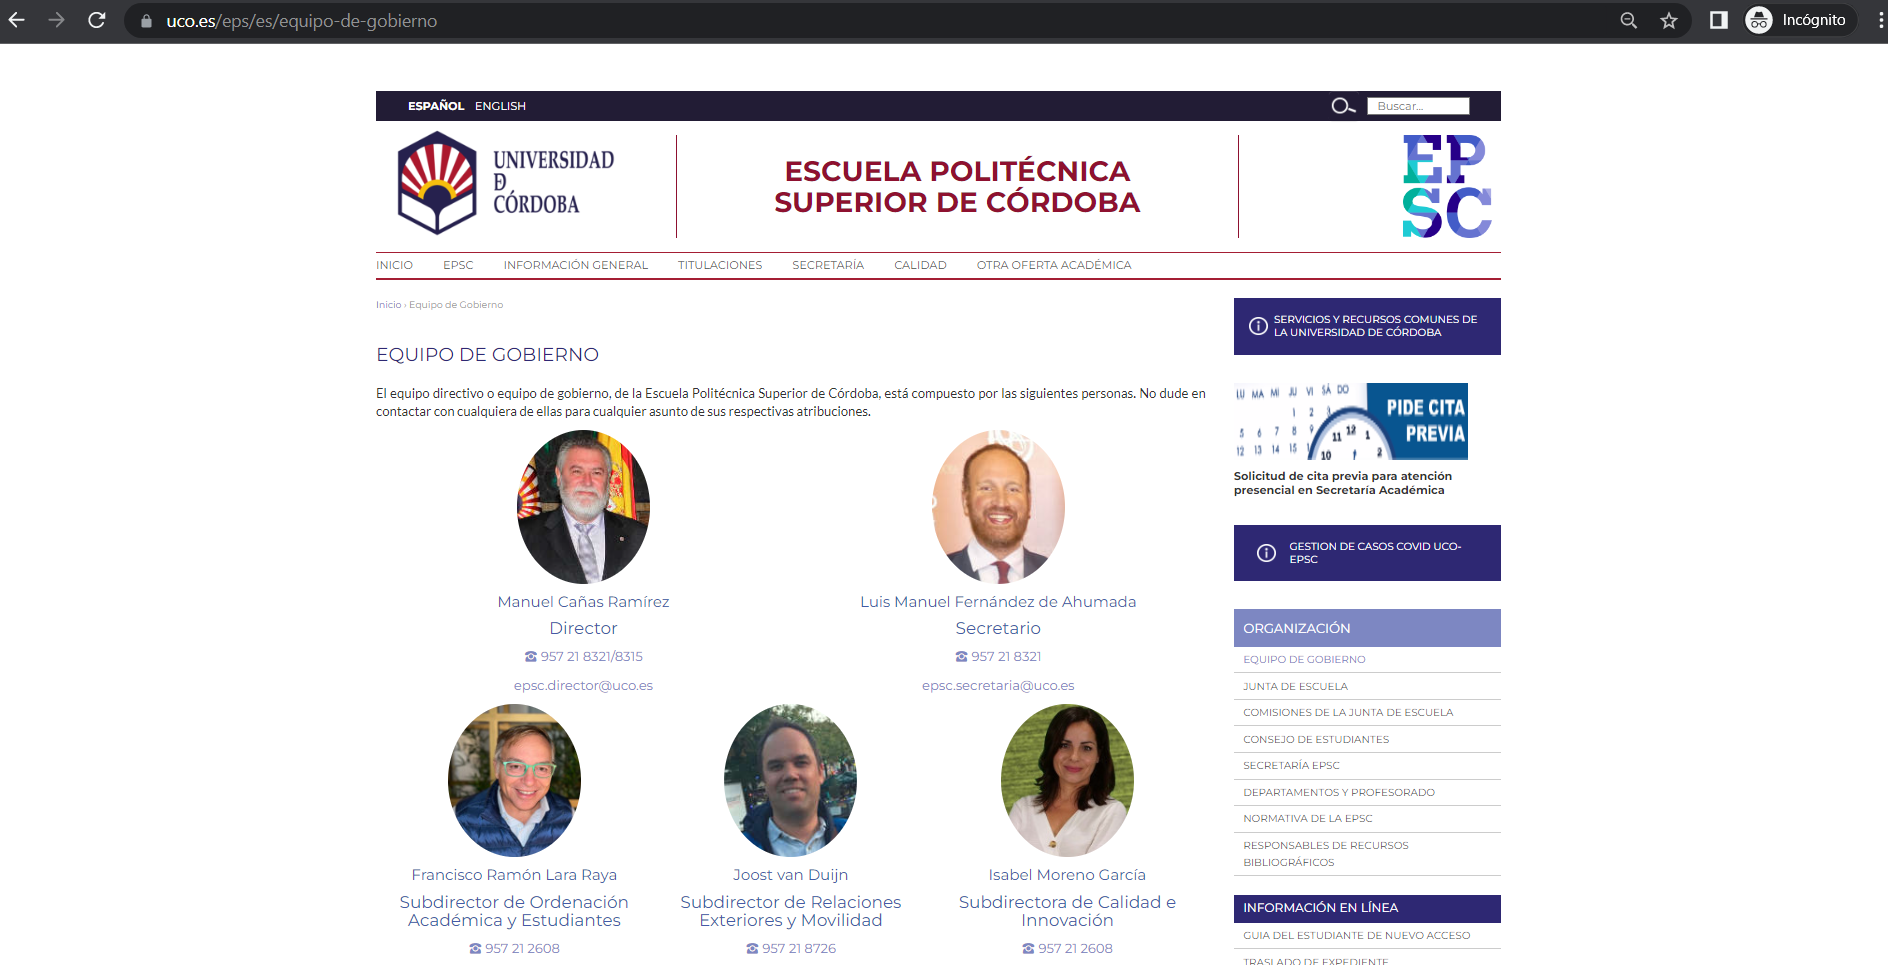
\includegraphics[scale=0.4]{img/capturas/WebEquipoGobiernoEPSUCO.png}
    \caption{WEB: equipo de gobierno de la EPS de la UCO}
    \label{fig:PACE-WebEquipoGobiernoEPSUCO}
\end{figure}

En definitiva, la Universidad de Córdoba carece de una aplicación web con una base de datos que permita asegurar la integridad de la información y evitar datos duplicados, ausentes o incorrectos. En la actualidad, se utilizan páginas web estáticas que deben ser mantenidas de forma individual, lo que provoca una gran carga de trabajo a los administrativos de los centros.

\section{Justificación del Trabajo de Fin de Grado}

El desarrollo del presente Trabajo de Fin de Grado está justificado porque no se tiene conocimiento de ninguna aplicación web que permita la gestión de comisiones de los distintos centros de la Universidad de Córdoba.

Actualmente, se realizan tareas manuales y estáticas sobre estas comisiones que provocan que la gestión administrativa sobre ellas sea una tarea lenta de realizar, sin conseguir una trazabilidad de cada uno de los cambios que pueden producirse a lo largo del tiempo y que repercute directamente en una pérdida de tiempo con respecto a utilizar un sistema que automatice lo máximo posible alguna de sus gestiones.

\chapter{Fase de Desarrollo}\label{c-fasedesarrollo}


El desarrollo del presente Trabajo de Fin de Grado va estar compuesto por la siguientes fases:

\begin{itemize}
     \item Introducción: descripción del problema, establecimiento de los objetivos, revisión de antecedentes, identificación de restricciones iniciales y estratégicas y selección de recursos.
     \item Análisis: especificación de requisitos (funcionales, no funcionales, de información y de la interfaz), descripción del modelo de datos y análisis funcional (casos de uso y diagramas de secuencia).
    
     \item Diseño: descripción del diseño de datos, clases, paquetes y de la interfaz.
    
     \item Implementación: codificación de la aplicación web teniendo en cuenta el diseño desarrollado.
    
     \item Pruebas: comprobación de que la aplicación web funciona correctamente, es robusta y amigable.
    
     \item Documentación: redacción del manual técnico (este documento), el manual de usuario y el manual de código.
 \end{itemize}
\chapter{Recursos}\label{cap:recursos}

\section{Recursos humanos}
\begin{itemize}
    \item \textbf{Autor}
    \item[] Javier Ruiz Jurado, estudiante del Grado en Ingeniería Informática, especialidad de Ingeniería del Software.
    \item \textbf{Director}
    \item[] José Luis Ávila Jiménez
\end{itemize}

\section{Recursos de hardware}

Para el desarrollo de la aplicación en el entorno local, se va a utilizar el equipo del alumno que tiene las características siguientes:
\begin{itemize}
    \item Ordenador: Acer Nitro 5
    \item Sistema operativo: Windows 11 Professional
    \item RAM instalada: 8GB DDR4
    \item Procesador: Intel(R) Core(TM) i7-10750H CPU @ 2.60GHz 
\end{itemize}

Para el despliegue de la aplicación web, se hará uso de un servidor VPS con las características siguientes:
\begin{itemize}
    \item Platform: Linux x86-64
    \item OS Package: Centos 7 (for AMD64/Intel EM64T) Virtuozzo Template
    \item Memory: 4.00 GB
    \item SSD: 50.00 GB
\end{itemize}


\section{Recursos de software}

Se van a utilizar los siguientes recursos de software para el desarrollo de la aplicación web: 
\begin{itemize}
    \item Editor de código fuente para el desarrollo de la aplicación web: Visual Studio Code \cite{visualStudioCode}
    \item \textit{Framework} utilizado para el desarrollo de la aplicación web, tanto en \textit{Back end} y \textit{Front end}: Laravel \cite{laravel}.
    \item Sistema de gestión de base de datos: MySql \cite{mysql}.
    \item Lenguajes de Programación: PHP \cite{PHP}, JavaScript \cite{javascript}.
    \item Redacción del documento: Overleaf \cite{overleaf}, editor en línea de documentos escritos en \LaTeX. 
    \item Editor de diagramas: draw.io \cite{drawio} y StarUML \cite{starUML}.
    \item Repositorio remoto en Github \cite{github}.
\end{itemize}



\chapter{Distribución Temporal}\label{c-distribuciontemporal}

La tabla \ref{tabla:distribucion-temporal} muestra el tiempo estimado para el desarrollo del presente Trabajo de Fin de Grado. El Reglamento de Trabajo Fin de Grado de la Escuela Politécnica Superior de Córdoba \cite{reglamentotfg} indica que el Trabajo de Fin de Grado debe tener una duración de 300 horas. 

\begin{table}[H]
    \centering
    \caption{Distribución temporal del Trabajo de Fin de Grado}\label{tabla:distribucion-temporal}
    \begin{tabular}{l|ccccc|r}
%\toprule
                     & Junio & Julio & Agosto & Septiembre & Octubre  & Total     \\ \hline
  Introducción         & 10 &  0  &  0  & 0  & 0  &  10  \\
  Análisis             & 10 & 40  &  0  & 0  & 0  &  50  \\
  Diseño               & 0  & 20  & 40  & 10 & 0  &  70  \\
  Implementación       & 0  & 10  & 30  & 40 & 10 &  90  \\
  Evaluación y pruebas & 0  &  0  &  0  & 10 & 20 &  30  \\
  Documentación        & 10 & 10  & 10  & 10 & 10 &  50  \\ \hline
  Total mes            & 30 & 80  & 80  & 70 & 40 & 300  
\end{tabular}
\end{table}

%\addcontentsline{toc}{chapter}{Referencias bibliográficas}
%\bibliography{references}
%\bibliographystyle{vancouver}
%\printbibheading[heading=bibintoc]
\printbibliography

\renewcommand{\appendixpagename}{Anexos}
\renewcommand{\appendixtocname}{Anexos}
\renewcommand{\appendixname}{Anexo}

\end{document}